\documentclass[12pt]{article}

\usepackage{sbc-template}
\usepackage{graphicx,url}
\usepackage{float}
\usepackage[brazil]{babel}
\usepackage[utf8]{inputenc}  

\sloppy

\title{Implementação dos métodos de verificação de similaridade de textos Dice's Coefficient e Longest Common Substring utilizando a linguagem de programação Racket}

\author{Vinícius da Costa Regatieri\inst{1}}

\address{Departamento de Informática -- Universidade Estadual de Maringá (UEM)\\
87.020-900 -- Maringá -- PR -- Brasil
\email{ra104016@uem.br}
}

\begin{document} 

\maketitle

\begin{abstract}
This paper aims to analyze and compare two text similarity checking methods, Dice's Coefficient and Longest Common Substring, both implemented in the Racket functional language. To this end, a set of eight texts, separated in pairs, was assembled and had beforehand calculated coefficients, taking into account both semantic and syntactic questions to serve as the basis of the study. As a result, the most accurate of the methods will be pointed out, as well as other ponderations.
\end{abstract}
     
\begin{resumo} 
Este trabalho tem como objetivo analisar e comparar dois métodos de verificação de similaridade de textos, Dice's Coefficient e Longest Common Substring, ambos implementados na linguagem funcional Racket. Para tal fim, um conjunto de oito textos, separados em pares foi montado e teve coeficientes previamente calculados, levando em consideração tanto questões semânticas, quanto questões sintáticas, para servirem de base do estudo. Como resultado, será apontado o mais acurado entre os métodos, assim como outras ponderações.
\end{resumo}

\section{Introdução}
A similaridade entre textos é discutida desde os primórdios das sociedades e está presente em várias comunidades científicas, desde linguistas até pesquisadores da área de computação. Com o avanço da tecnologia e dos computadores, cada vez mais se deseja passar o trabalho de comparação, seja ela semântica ou sintática, para as máquinas. Nesse contexto, muitas metodologias de comparação foram criadas ao longos dos anos, dentre elas, \textit{Longest Common Substring} e \textit{Dice's Coefficient}.

Esse trabalho tem como objetivo comparar a eficiência e a eficácia das duas metodologias supracitadas sobre um conjunto de textos utilizando a linguagem de programação funcional Racket. Para isso, faremos uma análise dos métodos utilizados e suas respectivas implementações e, após a execução das comparações, estudaremos os resultados obtidos para determinar sobre a eficiência e eficácia dos métodos.

\section{Métodos Utilizados}

Os dois métodos escolhidos para a realização deste trabalho foram ``\textit{Dice's Coefficient}"\ e ``\textit{Longest Common Substring}". A seguir, tais estratégias são descritas.

\subsection{Dice's Coefficient}

``Dice's Coefficient"\ é um método estatístico usado para medir a similaridade de duas amostras discretas quaisquer, não somente aplicado a textos. Para calcular o coeficiente, sua fórmula padrão é descrita como a seguir: 
\begin{equation}
DSC={\frac {2|X\cap Y|}{|X|+|Y|}}
\end{equation}
em que X e Y são conjuntos de dados.

Para aplicar o método à comparação de \textit{strings}, devemos primeiro encontrar os \textit{bigrams} dos textos fornecidos ao método. Um \textit{bigram} é um subconjunto de caracteres do texto de tamanho dois. Como exemplo, na palavra ``NOITE", após encontrados seus \textit{bigrams}, tem-se o conjunto $X=\{NO, OI, IT, TE\}$

O cálculo do coeficiente do método aplicado a textos se torna:

\begin{equation}
    DSC={\frac{2\alpha}{\beta_x + \beta_y}}
\end{equation}
em que $\alpha$ representa o número de \textit{bigrams} iguais em ambos os textos, $\beta_x$ representa o total de \textit{bigrams} no texto X e $\beta_y$ representa o total de \textit{bigrams} no texto Y. 

Segundo \cite{gomaa2013survey}, o método é caracterizado como uma medida de similaridade baseada em termos. Isso se deve ao fato de comparar subtermos do texto fornecido, nesse caso subtermos de tamanho 2, os \textit{bigrams}.

\subsection{Longest Common Substring}

``Longest Common Substring"\ é um método que consiste em encontrar a maior subsequência de caracteres de dois ou mais textos, muito comum na área da Ciência da Computação. Segundo \cite{gomaa2013survey}, é caracterizado como uma medida de similaridade baseada em caracteres pelo fato de se basear no tamanho do maior encadeamento de caracteres que existem nos textos, portanto comparando cada caractere nas duas \textit{strings}.

Por retornar o tamanho da maior subsequência de caracteres, para o método ter como resultado um número entre 0 e 1 foi preciso normalizar o valor gerado pelo algoritmo implementado, como descrito a seguir:

\begin{equation}
    LCS={\frac{\alpha}{max(\beta_x , \beta_y)}}
\end{equation}
em que $\alpha$ representa a solução gerada pelo algoritmo LCS, ou seja, o tamanho da maior cadeia de caracteres iguais nos textos, $\beta_x$ representa o tamanho do texto X, $\beta_y$ representa o tamanho do texto Y e a função $max(a, b)$ retorna o maior entre os parâmetros a e b.

\section{Metodologia} \label{sec:metodologia}
Para a avaliação das metodologias propostas, um conjunto de oito textos será criado. Estes textos serão executados aos pares em ambos os algoritmos desenvolvidos e os coeficientes gerados serão armazenados em uma tabela. Cada par de textos terá uma medida de similaridade previamente calculada, referida a partir daqui como padrão-ouro, com base nas suas semelhanças semânticas ou sintáticas.

Após a execução dos quatro casos de teste, uma tabela com os valores dos coeficientes calculados de cada par de textos em cada algoritmo e seu valor previamente medido será obtida. Para definir a relação entre os resultados de um algoritmo e os valores ``padrão-ouro", uma correlação estatística simples será calculada. Dessa forma, o algoritmo que apresentar correlação mais próxima de 1 (um) será dito como mais acurado na verificação de similaridade de textos.

Os pares de textos a serem utilizados nos testes têm as seguintes características:

\begin{itemize}
    \item O par 1-5 tem exatamente o mesmo conteúdo. Por esse motivo o padrão-ouro calculado é 1,00;
    \item O par 2-6 tem textos com significados totalmente diferentes. Nesse contexto, apesar de possivelmente possuírem palavras iguais, o padrão-ouro calculado é 0,00;
    \item O par 3-7 é um caso que representa a cópia de um parágrafo em um trabalho acadêmico. Nesse caso, sessenta e uma palavras teriam sido plagiadas, tornando 37\% do texto semelhante sintaticamente. Padrão-ouro calculado de 0,37\footnote{O cálculo de plágio foi feito com o auxílio do site Copyleaks: \url{https://copyleaks.com/}};
    \item O par 4-8 tem duas frases isoladas com metade das palavras iguais. Nesse caso, padrão-ouro calculado de 0,5.
\end{itemize}

\section{Avaliação e discussão} \label{sec:avaliacao}

Executados todos os testes e cálculos propostos na seção \ref{sec:metodologia}, foi possível obter a seguinte tabela de resultados:

\begin{table}[H]
\centering
\begin{tabular}{|c|c|c|c}
\hline
 & Dice's Coefficient & LCS & \multicolumn{1}{c|}{Padrão-Ouro} \\ \hline
Textos 1/5 & 1,00 & 1,00 & \multicolumn{1}{c|}{1,00} \\ \hline
Textos 2/6 & 0,59 & 0,34 & \multicolumn{1}{c|}{0,00} \\ \hline
Textos 3/7 & 0,94 & 0,43 & \multicolumn{1}{c|}{0,37} \\ \hline
Textos 4/8 & 0,59 & 0,78 & \multicolumn{1}{c|}{0,50} \\ \hline
\multicolumn{1}{|l|}{\textbf{Correlação}} & 0,67 & 0,94 & \multicolumn{1}{l}{} \\ \cline{1-3}
\end{tabular}
\caption{Tabela de resultados}
\label{tab:resultados}
\end{table}

Analisando a tabela \ref{tab:resultados}, é possível observar que a maior correlação com o padrão-ouro é do método \textit{Longest Common Substring}. Isso se deve ao fato de que seu concorrente, \textit{Dice's Coefficient}, procura por bigramas correspondentes, o que o faz enaltecer padrões nos textos, fato comprovado pelo resultado muito próximo de 1 do par de textos 3-7, enquanto ele, LCS, funciona melhor para sistemas de revisão de controle, como por exemplo git, por conseguir quantificar o número de alterações nos textos.

Além da correlação com o padrão-ouro, é importante verificarmos o tempo de execução dos algoritmos. A figura \ref{fig:exec-time} contém tais dados:

\begin{figure}[H]
    \centering
    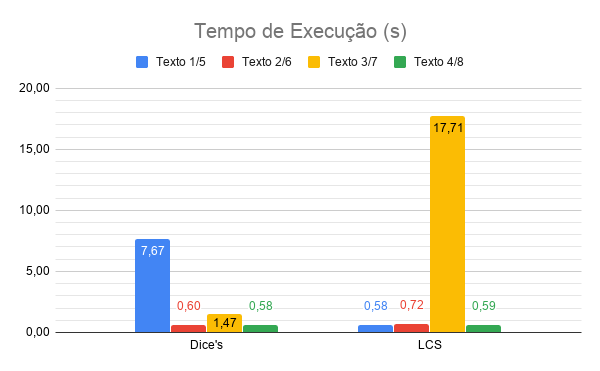
\includegraphics[scale=0.65]{exec-time.png}
    \caption{Tempo de execução dos algoritmos para cada par de texto}
    \label{fig:exec-time}
\end{figure}

É possível enxergar os grandes \textit{outliers} existentes no cálculo do coeficiente pelo método LCS par de textos 3-7, e pelo método \textit{Dice's Coefficient} no par 1-5. Com isso, a média do tempo de execução dos algoritmos foi $2,58 s$ e $4,90 s$ para o método \textit{Dice's} e LCS, respectivamente. Com o resultado, é certo afirmar que, no quesito tempo de execução, o algoritmo \textit{Dice's Coefficient} se mostra vantajoso para um caso médio. 

Essa vantagem no tempo de execução pode ser explicada pela técnica usada na construção do algoritmo, que é baseada em termos e, como o próprio nome já diz, baseia-se em conjuntos de caracteres, de tamanho dois, nesse caso, para fazer suas computações, o que acaba diminuindo a quantidade de comparações necessárias no melhor e médio casos. 

O pior caso do algoritmo de Dice está no caso em que todos os bigramas são iguais, o que pode ser visto no teste do par 1-5, explicando seu resultado acima da média.

\section{Conclusão}

O desenvolvimento do presente trabalho possibilitou um melhor entendimento de dois métodos de verificação de similaridades em textos, área crescente tanto no contexto acadêmico, quanto empresarial.

Como discutido na seção \ref{sec:avaliacao}, ``avaliação e discussão", o algoritmo \textit{Longest Common Substring} se mostrou mais acurado na verificação de similaridade de textos levando em consideração a metodologia deste estudo. Isso mostra que a técnica de comparação por caracteres consegue captar contexto, ainda que de modo sutil.

Não podemos, todavia, descartar a importância do outro método abordado no trabalho, \textit{Dice's Coefficient}. Sua técnica de comparação por termos se mostra muito útil em situações que se pretende valorar similaridades léxicas ou encontrar padrões, como no campo genético da biologia.

Trabalhos futuros complementares podem incluir comparações de implementações dos métodos apresentados neste trabalho nos diferentes paradigmas de programação a fim de medir seu custo-benefício e comparações de outros métodos baseados em caracteres e o método \textit{Longest Common Substring} com o objetivo de determinar melhores algoritmos de verificação de similaridades nesse contexto.

\bibliographystyle{sbc}
\bibliography{sbc-template}

\end{document}
